\documentclass{article}

\usepackage{graphicx}
\usepackage{tikz}
\usepackage{tikzsymbols}
\usetikzlibrary{calc,patterns,shapes.geometric}
\pagestyle{empty}
\usepackage[margin=0pt]{geometry}
\geometry{papersize={14in,12in}}

\def\centerarc[#1](#2)(#3:#4:#5){\draw[#1] ($(#2)+({#5*cos(#3)},{#5*sin(#3)})$) arc (#3:#4:#5);}

\begin{document}
	\begin{figure}
		\centering
		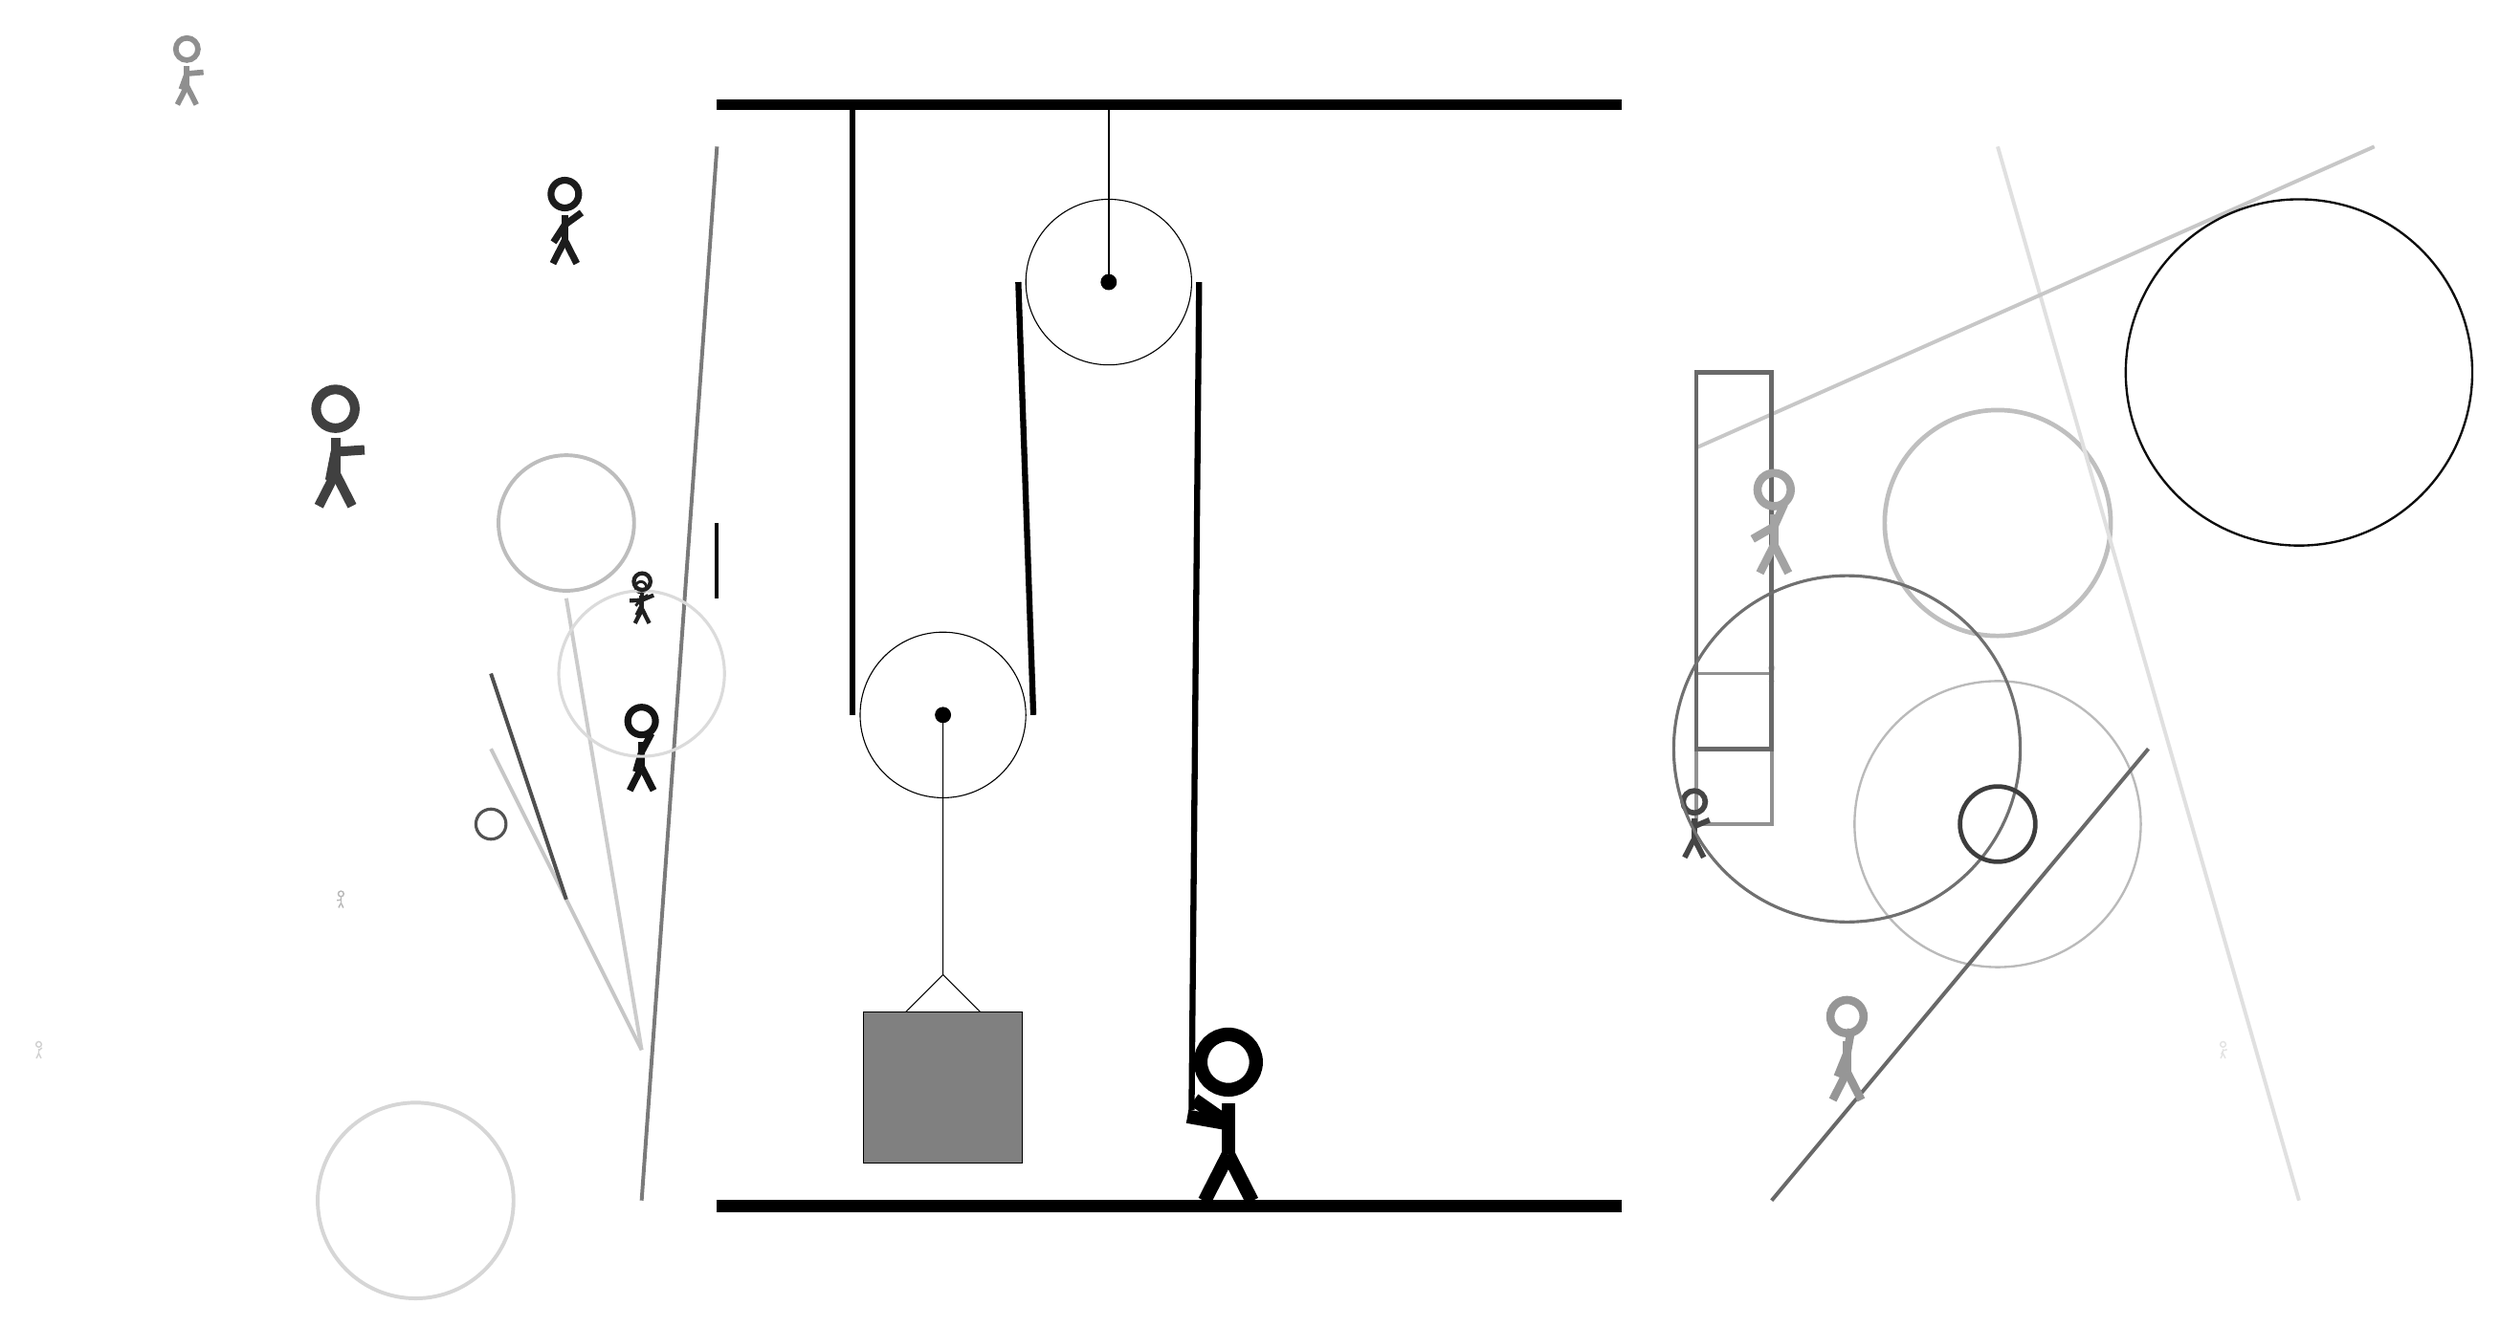
\begin{tikzpicture}
			%%%%% START %%%%%
			
			\draw[fill=black] (-2, 11.5) rectangle (10, 11.625);
			
			\draw (3.2, 9.2) circle (1.1);
			\draw[fill=black] (3.2, 9.2) circle (0.1);
			\draw[thick] (3.2, 9.2) -- (3.2, 11.5);
			
			\draw (1, 3.45) circle (1.1);
			\draw[fill=black] (1, 3.45) circle (0.1);
			
			\draw (1, 3.45) -- (1, 0.0) -- (0.5, -0.5);
			\draw (1, 0.0) -- (1.5, -0.5);
			\draw[fill=black!50] (-0.05, -0.5) rectangle (2.05, -2.5);
			
			\draw[line width=0.8mm] (-0.2, 11.5) -- (-0.2, 3.45);
			\centerarc[line width=0.8mm](1, 3.45)(180:360:1.2000000000000002);
			\draw[line width=0.8mm](2.2, 3.45) -- (2.0, 9.2);
			\centerarc[line width=0.8mm](3.2, 9.2)(0:180:1.2000000000000002);
			\draw[line width=0.8mm](4.4, 9.2) -- (4.3, -1.8);
			
			\node at (4.7, -1.9) {\Strichmaxerl[10][-35][170]};
			
			\draw [line width=0.3mm, color=black!27](15, 2) circle (1.9);
			
			\draw[line width=0.5mm, color=black!100] (-2, 6) rectangle (-2, 5);
			\draw[line width=0.5mm, color=black!20](-3, -1) -- (-4, 5);
			\node[line width=0.2mm, color=black!11] at (18, -1) {\Strichmaxerl[1][65][14]};
			\node[line width=0.4mm, color=black!20] at (12, 4) {\Strichmaxerl[1][85][84]};
			\draw [line width=0.6mm, color=black!25](15, 6) circle (1.5);
			\node[line width=0.4mm, color=black!87] at (-3, 5) {\Strichmaxerl[2][51][32]};
			\draw[line width=0.5mm, color=black!22](-3, -1) -- (-5, 3);
			\draw [line width=0.5mm, color=black!16](-6, -3) circle (1.3);
			\draw[line width=0.5mm, color=black!43] (11, 2) rectangle (12, 4);
			\draw[line width=0.5mm, color=black!12](15, 11) -- (19, -3);
			
			\node[line width=0.6mm, color=black!44] at (-9, 12) {\Strichmaxerl[4][70][5]};
			\draw[line width=0.5mm, color=black!69](-4, 1) -- (-5, 4);
			
			\node[line width=0.3mm, color=black!18] at (-11, -1) {\Strichmaxerl[1][89][40]};
			\draw[line width=0.5mm, color=black!22](11, 7) -- (20, 11);
			\draw[line width=0.6mm, color=black!59] (12, 3) rectangle (11, 8);
			
			\node[line width=0.7mm, color=black!89] at (-4, 10) {\Strichmaxerl[5][57][36]};
			\draw[line width=0.5mm, color=black!52](-2, 11) -- (-3, -3);
			\node[line width=0.4mm, color=black!28] at (-7, 1) {\Strichmaxerl[1][4][88]};
			\draw [line width=0.4mm, color=black!68](-5, 2) circle (0.2);
			\draw[line width=0.5mm, color=black!59](12, -3) -- (17, 3);
			\draw [line width=0.5mm, color=black!26](-4, 6) circle (0.9);
			
			\node[line width=0.4mm, color=black!75] at (-7, 7) {\Strichmaxerl[7][79][4]};
			\node[line width=0.3mm, color=black!92] at (-3, 3) {\Strichmaxerl[5][74][62]};
			\draw [line width=0.4mm, color=black!14](-3, 4) circle (1.1);
			
			\node[line width=0.3mm, color=black!73] at (11, 2) {\Strichmaxerl[4][90][23]};
			\node[line width=0.5mm, color=black!36] at (12, 6) {\Strichmaxerl[6][30][66]};
			\draw [line width=0.4mm, color=black!56](13, 3) circle (2.3);
			\node[line width=0.4mm, color=black!41] at (13, -1) {\Strichmaxerl[6][68][80]};
			\node[line width=0.7mm, color=black!87] at (-3, 5) {\Strichmaxerl[3][3][23]};
			\draw [line width=0.3mm, color=black!95](19, 8) circle (2.3);
			
			\draw [line width=0.6mm, color=black!76](15, 2) circle (0.5);
			
			\draw[fill=black] (-2, -3) rectangle (10, -3.15);
			
			%%%%% END %%%%%
		\end{tikzpicture}
	\end{figure}	
\end{document}